% =============================================================================
% Section 3 — The No-Go Theorem
% =============================================================================
\section{A No-Go Theorem for Stage-Removal Models}\label{sec:nogo}

\begin{objectives}
\begin{itemize}[leftmargin=*,itemsep=1pt,topsep=1pt]
  \item State the stage-removal model class precisely enough that it can be refuted.
  \item Prove that every member of the class obeys a ceiling, with no fitted parameter.
  \item Use the contrapositive to turn a measured excess into a constraint on the enzyme.
  \item Explain why a theorem with no free parameters is worth more than one with many.
\end{itemize}
\end{objectives}

\subsection{The question}

Section~2 gave a model in which fidelity comes from $m$ multiplicative stages.
A natural hypothesis about a mutator allele --- one that produces more mutations
than wild type --- is that it has \emph{lost} some of those stages. Call this a
\textbf{stage-removal} hypothesis. It is attractive: it explains a mutator
phenotype with no new machinery, only subtraction.

This section asks how far such a hypothesis can go, and the answer is: not far
enough. There is a ceiling, it is low, and it holds for every model of this shape.

\subsection{The model class}

\begin{model}[Stage-removal class]\label{model:class}
Let $\inserr > 0$ be the \emph{insertion/extension error}: the rate at which the
polymerase incorporates a wrong nucleotide before any proofreading acts. Let the
enzyme possess a finite set $\stages$ of proofreading stages, stage $i$ letting an
error escape with probability $\escape_i \in [0,1]$. The error rate is
\begin{equation}\label{eq:errorrate}
  \errate(\stages) \;=\; \inserr \prod_{i \in \stages} \escape_i .
\end{equation}
A \emph{stage-removal mutant} retains a subset $\kept \subseteq \stages$ and changes
nothing else: same $\inserr$, same $\escape_i$ on the stages it keeps.
\end{model}

This class is broad. Section~2's cascade is the special case $\escape_i \equiv \gamma$,
giving $\errate = \inserr\gamma^{m}$. Exonuclease-partitioning models, where a
fraction $p_{\mathrm{exo}}$ of errors is excised, are the case
$\escape_i = 1 - p_{\mathrm{exo}}$. Any scheme in which independent filters act in
series and the mutant differs only by having fewer of them is covered.

Note the empty product convention: an enzyme with no stages at all has
$\errate(\emptyset) = \inserr$. Biologically this is the \textbf{exonuclease-null}
enzyme --- proofreading entirely absent. It will be the reference point.

\subsection{The theorems}

\begin{theorem}[Monotonicity, PSR$_1$]\label{thm:psr1}
Let $\inserr \ge 0$ and $\escape_i \in [0,1]$ for all $i$. If $\kept \subseteq \stages$ then
$\errate(\stages) \le \errate(\kept)$.
\end{theorem}

\begin{proof}
Partition the product over $\stages$ into the stages kept and the stages dropped:
\[
  \prod_{i \in \stages} \escape_i
  \;=\; \Big(\prod_{i \in \kept} \escape_i\Big)\Big(\prod_{i \in \stages \setminus \kept} \escape_i\Big).
\]
Every factor lies in $[0,1]$, so the second bracket lies in $[0,1]$, and the first
is non-negative. Hence $\prod_{i\in \stages}\escape_i \le \prod_{i \in \kept}\escape_i$.
Multiplying by $\inserr \ge 0$ preserves the inequality.
\end{proof}

\begin{theorem}[The ceiling, PSR$_2$]\label{thm:psr2}
Under the same hypotheses, $\errate(\kept) \le \inserr$ for every $\kept$. No
stage-removal mutant can exceed the exonuclease-null error rate.
\end{theorem}

\begin{proof}
$\prod_{i \in \kept} \escape_i \le 1$, being a product of factors in $[0,1]$. Multiply
by $\inserr \ge 0$.
\end{proof}

\begin{theorem}[Contrapositive, PSR$_3$]\label{thm:psr3}
Suppose a variant is measured at $\rho$ times the exonuclease-null rate, with
$\rho > 1$. Then its insertion error $\inserr'$ satisfies $\inserr' \ge \rho\,\inserr$:
whatever stages it keeps, it is not a stage-removal mutant.
\end{theorem}

\begin{proof}
By Theorem~\ref{thm:psr2} applied with insertion error $\inserr'$, the variant's
rate is at most $\inserr'$. If that rate equals $\rho\inserr$ then
$\rho\inserr \le \inserr'$.
\end{proof}

\begin{remark}[What makes this worth proving]\label{rem:nofit}
Observe what Theorem~\ref{thm:psr2} does \emph{not} contain: a stage count, a
value of $\gamma$, a fitted constant, a free parameter of any kind. It is a bound
on an entire family of models, uniform over everything the family could be tuned
to. That is why a single measurement can refute it --- and why, if the
measurement had fallen below the ceiling, we would have learned almost nothing.
A theorem's value as evidence is set by how easily it could have failed.
\end{remark}

\subsection{Formalisation}

In \file{formal/ANSE/ProofreadingStageRemoval.lean}. The error rate is a
\lean{Finset} product, so ``removing stages'' is literally passing to a subset.

\begin{lstlisting}
noncomputable def errorRate {ι : Type*} (ε : ℝ) (q : ι → ℝ) (S : Finset ι) : ℝ :=
  ε * ∏ i ∈ S, q i

theorem PSR_1_stage_removal_monotone {ι : Type*} [DecidableEq ι] (ε : ℝ) (hε : 0 ≤ ε)
    (q : ι → ℝ) (h0 : ∀ i, 0 ≤ q i) (h1 : ∀ i, q i ≤ 1) {T S : Finset ι} (hTS : T ⊆ S) :
    errorRate ε q S ≤ errorRate ε q T := by
  unfold errorRate
  exact mul_le_mul_of_nonneg_left (prod_subset_ge q hTS h0 h1) hε
\end{lstlisting}

The file declares seven items --- the three theorems, two supporting lemmas about
products, and two controls --- and all seven pass the axiom gate with no
\lean{sorryAx}. The controls matter: \lean{PSR_positive_control} exhibits a
configuration satisfying the hypotheses, so the theorems are not vacuous, and
\lean{PSR_negative_control} exhibits a $\escape_i > 1$ for which the ceiling
genuinely fails, confirming that the range hypothesis is load-bearing rather than
decorative.

\begin{figure}[htbp]
  \centering
  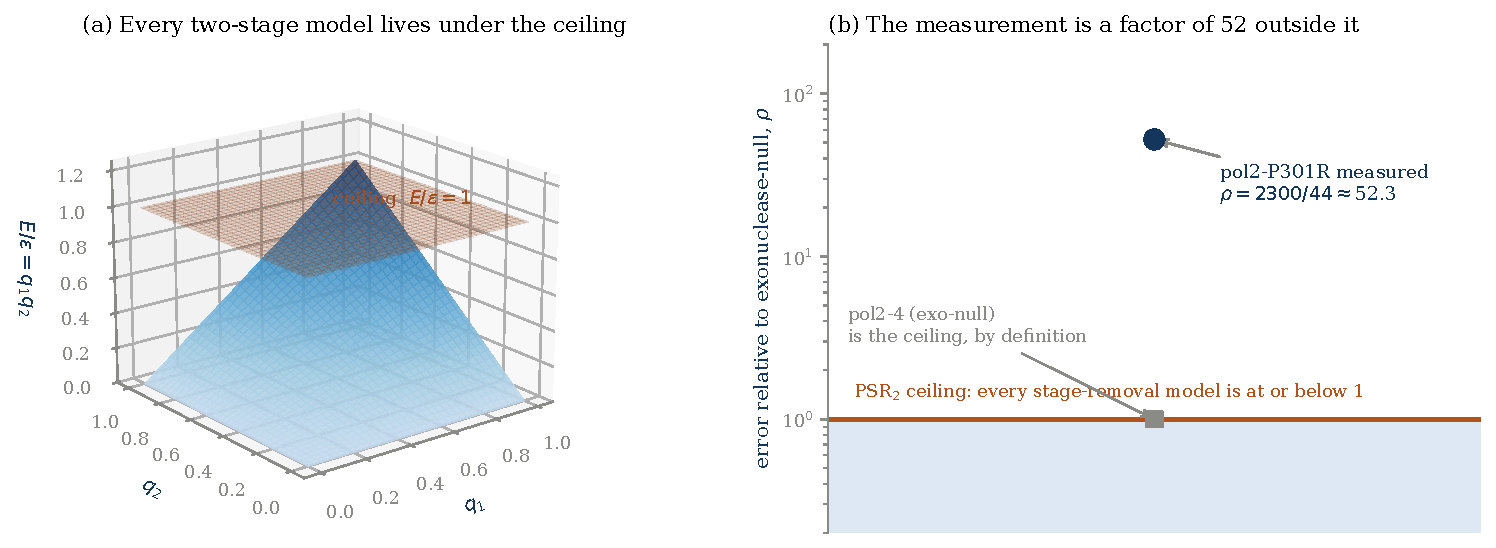
\includegraphics[width=\textwidth]{fig03_nogo_ceiling.pdf}
  \caption{(a) The feasible region for a two-stage model. The blue surface is
  $\errate/\inserr = \escape_1\escape_2$ over $[0,1]^2$; the flat orange plane is the ceiling
  $\errate/\inserr = 1$. Every point of the surface lies at or below the plane, and
  that remains true for any number of stages --- which is
  Theorem~\ref{thm:psr2}. (b) The same bound on a logarithmic axis, with the
  measurement of Section~\ref{sec:refutation} placed on it. The shaded band is
  everything the model class permits.}
  \label{fig:ceiling}
\end{figure}

\begin{worked}[3.1: the ceiling cannot be escaped by adding stages]
\textbf{Problem.} A colleague proposes rescuing the stage-removal hypothesis by
positing that wild type has not three but twenty proofreading stages, so that
losing nineteen of them produces a huge effect. Evaluate the proposal.

\textbf{Solution.} It changes nothing. Theorem~\ref{thm:psr2} bounds
$\errate(\kept) \le \inserr$ for \emph{every} subset $\kept$, including $\kept = \emptyset$.
Adding stages to the wild type lowers $\errate(\stages)$ --- making the mutant's
\emph{relative} excess over wild type larger --- but the comparison that matters
is against the exonuclease-null rate $\inserr$, and no subset can exceed it.
The proposal confuses two ratios:
\[
  \underbrace{\frac{\errate(\kept)}{\errate(\stages)}}_{\text{unbounded}}
  \qquad\text{versus}\qquad
  \underbrace{\frac{\errate(\kept)}{\inserr}}_{\le\,1\ \text{always}} .
\]
The first can be made as large as you like by giving wild type more stages. The
second is capped. Section~\ref{sec:refutation} measures the second, which is why
the measurement bites.
\end{worked}

\begin{exercise}
Prove that $\errate(\kept) \le \inserr$ directly from Theorem~\ref{thm:psr1} by
choosing $\stages = \kept$ and $\kept = \emptyset$ appropriately. (This shows
PSR$_2$ is a corollary of PSR$_1$; the Lean file proves it independently so that
each can be cited alone.)
\end{exercise}

\begin{exercise}
Identify which of Assumption~\ref{model:class}'s requirements fails in each
scenario, and whether the ceiling survives.
\textbf{(a)} A stage that, when retained, makes a \emph{different} stage less
effective. \textbf{(b)} A mutant whose insertion error is larger than wild type's.
\textbf{(c)} A ``stage'' modelled with $\escape_i = 1.4$.
\end{exercise}

\begin{exercise}
Remark~\ref{rem:nofit} claims a parameter-free theorem is better evidence than a
tunable one. Make this precise: let $M_\theta$ be a family of models indexed by
$\theta \in \Theta$, and define what it means for an observation to refute the
family rather than a member. Why does enlarging $\Theta$ weaken the family's
empirical content?
\end{exercise}

\begin{ledger}
\textbf{Measured:} nothing in this section; it is pure theory. The measurement
arrives in Section~\ref{sec:refutation}. \\
\textbf{Assumed:} Assumption~\ref{model:class} --- multiplicative composition,
per-stage factors in $[0,1]$, and a mutant that differs from wild type only by
which stages it retains. \\
\textbf{Proved:} Theorems~\ref{thm:psr1}--\ref{thm:psr3}
(\lean{PSR_1_stage_removal_monotone}, \lean{PSR_2_bounded_by_exo_null},
\lean{PSR_3_excess_over_exo_null_forces_insertion_defect}), with positive
and negative controls. Gate: 7 of 7 declarations clean, no \lean{sorryAx},
axioms within $\{$\lean{propext}, \lean{Classical.choice}, \lean{Quot.sound}$\}$. \\
\textbf{Open:} whether any real cooperative mechanism could supply the
interaction that \S\ref{sub:interact} shows a rescue would need. That is a
question for enzymology, and this book does not answer it. \\
\textbf{Closed in this edition:} the class assumes stages act independently, and
the first edition left the interacting case entirely untreated. It is now
treated: \S\ref{sub:interact} carries an explicit interaction factor $\Lambda$,
proves the ceiling becomes $\inserr\Lambda$ (Theorem~\ref{thm:psr2i}), and shows
that the measured ratio forces $\Lambda \ge 52.3$
(Theorem~\ref{thm:psr3i}). The escape route is open but priced, which is a
better outcome than either ignoring it or pretending it is closed.
\end{ledger}
